

Da questo capitolo in poi esamino uno a uno i requisiti base dell'applicazione, spiegando per ognuno
i problemi riscontrati le soluzioni proposte e implementate per soddisfarli.

Avendo definito i principali metodi di navigatione tra ViewController al capitolo~\ref{CH:2} torniamo al problema iniziale:
\textit{Come possiamo rendere dinamica la navigazione?}

A seguito di uno studio approfondito di varie tecniche di navigazione iOS ho scelto di utilizzare il
\textbf{Coordinator Pattern}\cite{coordinatorpattern}.

\section{Il Coordinator Pattern}\label{sec:coordinator}

Generalmente in iOS l'intera logica di un ViewController viene scritta nel controller stesso, creando spesso
file di grosse dimensioni e disordine generale. Il Coordinator Pattern è nato proprio per rendere 
le applicazioni più scalabili e leggere. 

Ogni ViewController infatti delega tutte le decisioni al suo Coordinator usando il Delegation Pattern (vedere sezione~\ref{delegation}) che in base alle logiche
della vista in questione deciderà i passi successivi.

Ogni Coordinator può controllare un ViewController o più Coordinator. Questo rende le viste
indipendenti tra di loro e rende ogni ViewControler totalmente invisibile agli altri.\\

\begin{minipage}{\linewidth}
    \centering
    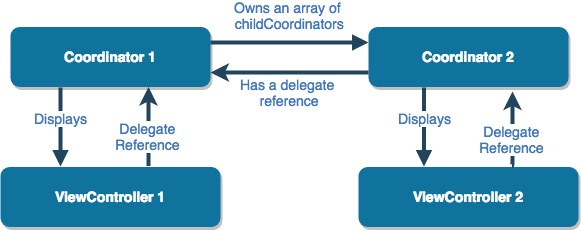
\includegraphics[width=10cm]{coordinator}
    \captionof{figure}{
        Il Coordinator Pattern
    }
    \label{fig:4}
\end{minipage} \\\\ 

La resposibilità dei coordinator è infatti la navigazione. Come un navigation controller gestisce i sui View Controller, un coordinator gestisce
i suoi figli e questo rende ogni vista o flow di navigazione totalmente indipendente dal resto dell'applicazione.

Per navigare tra i view controller vengono generalmente usate le tipologie di navigazione
descritte nella sezione~\ref{sec:navigation}, tranne le segue, che essendo definite da vista grafica renderebbero
la navigazione statica e fissata su determinati ViewController. \\

Di seguito in figura~\ref{fig:5} presento uno schema dell'utilizzo di due coordinator
per la gestione di una lista di prodotti e il carrello. \\

\begin{minipage}{\linewidth}
    \centering
    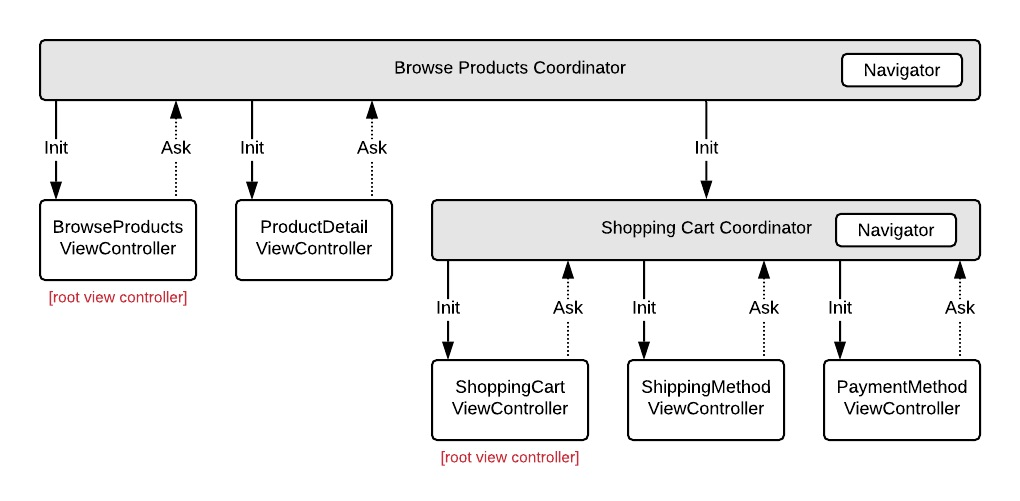
\includegraphics[width=10cm]{coordinator-example}
    \captionof{figure}{
       Esempio di coordinator pattern
    }
    \label{fig:5}
\end{minipage} \\\\

Come si evince dalla figura~\ref{fig:5} è presente in entrambi i coordinator un oggetto
\textbf{navigator} che sarà il proxy di un generico UINavigationController

\section{Implementazione}

Ogni coordinator ha degli elementi fissi che sono:

\begin{itemize}
    \item Una funzione di partenza denominata \textbf{start};
    \item Un array di coordinator figli;
\end{itemize}

Per questo ho iniziato implementando dei protocolli che sono descritti nelle sezioni seguenti.
\subsection{Protocolli base}

Il primo protollo implementato è quello che definisce un qualunque coordinator
e ne tiene in memoria i figli in modo che non vengano
deallocati automaticamente dal sistema operativo.

\begin{minted}{swift}
protocol Coordinator: class {

    var childCoordinators: [Coordinator] { get set }
    
    /** Utilizzato task di inizializzazione */
    func start()
    
}

extension Coordinator {
    
    // Aggiunge un figlio al coordinator padre
    func add(childCoordinator: Coordinator) {
        childCoordinators.append(childCoordinator)
    }
    
    // Rimuove un Coordinator figlio dal parent
    func remove(childCoordinator: Coordinator) {
        childCoordinators = childCoordinators.filter {
            $0 !== childCoordinator 
        }
    }
}
\end{minted}

Successivamente è stato implementato un BaseCoordinatorPresentable, che estende Coordinator
e aggiunge delle funzionalità di presentazione modale.

\begin{minted}{swift}
protocol BaseCoordinatorPresentable: Coordinator {

    // Il view controller principale del coordinator
    var _rootViewController: UIViewController { get }
}

// MARK: - Presentation Methods

extension BaseCoordinatorPresentable {
    
    /**
     Inizia un coordinator figlio e presenta
     il suo rootViewController modalmente

     - Parametri:
        - childCoordinator: Il coordinator da presentare
        - animated: Specifica se con o senza animazione modale
     */
    
    func presentCoordinator(_ childCoordinator:
        BaseCoordinatorPresentable, animated: Bool) {

        add(childCoordinator: childCoordinator)
        childCoordinator.start()
        _rootViewController.present(
            childCoordinator._rootViewController,
            animated: animated
        )
    }
    
    /**
     Inizia un viewController senza coordinator e
     lo presenta modalmente
     
     - Parametri:
        - controller: Il controller da presentare
        - animated: Specifica se con o senza animazione modale
     */
    
    func present(_ controller: UIViewController, animated: Bool) {
        _rootViewController.present(controller, animated: animated)
    }
    
    /**
     Interrompe la presentazione di un child Coordinator
     eliminandolo anche dall'array in memoria

     - Parameters:
        - childCoordinator: Il coordinator da chiudere e rilasciare
        - animated: Specifica se con o senza animazione modale
        - completion: closure che viene eseguita alla vine 
          del dismiss
     */
    
    func dismissCoordinator(_ childCoordinator:
        BaseCoordinatorPresentable,
        animated: Bool, completion: (() -> Void)? = nil) {

        childCoordinator._rootViewController.dismiss(animated: animated,
            completion: completion)
        self.remove(childCoordinator: childCoordinator)
    }

}
\end{minted}

\subsection{Coordinator modale}

Il BaseCoordinatorPresentable è stato definito per evitare errori di \textbf{associetedtype},
infatti questo protocollo non deve mai essere implementato direttamente, ma soltanto con il protocollo successivo

\begin{minted}{swift}
protocol CoordinatorPresentable: BaseCoordinatorPresentable {

    /**
        Questo protocolo utilizza la tipizzazione per
        permettere di ottenere Coordinator con view
        controller tipizzati.
     */
    associatedtype ViewController: UIViewController

    // Il rootViewController del coordinator
    var rootViewController: ViewController { get }

}

extension CoordinatorPresentable {

    // Ritorna rootViewController
    var _rootViewController: UIViewController {
        return rootViewController
    }
}
\end{minted}

\section{Aggiunta del Navigator}

Successivamente ho creato un protocollo \textbf{CoordinatorNavigable} che estende 
il coordinator visto in precedenza e ne aggiunge un oggetto navigator

\begin{minted}{swift}
protocol CoordinatorNavigable: CoordinatorPresentable {
    
    /** Responsabile dello stack di navigazione  */
    var navigator: Navigator { get }
}

extension CoordinatorNavigable {
    
    /**
     Aggiunge il rootViewController allo stack di navigazione
    */
    func pushCoordinator(_ childCoordinator:
        BaseCoordinatorPresentable, animated: Bool) {

        add(childCoordinator: childCoordinator)
        childCoordinator.start()
        navigator.push(childCoordinator._rootViewController,
                animated: animated,
                onPoppedCompletion: { [weak self] in
                    self?.remove(childCoordinator: childCoordinator)
        })
    }
}

final class Navigator: NSObject {

    private let navigationController: UINavigationController
    private var completions: [UIViewController: () -> Void]
    
    init(navigationController:
        UINavigationController = UINavigationController()) {
            
        self.navigationController = navigationController
        self.completions = [:]
        
        super.init()
        
        self.navigationController.delegate = self
    }
}
\end{minted}

Come si può osservare dall'esempio riportato precedentemente il \textbf{Navigator}
ha lo scopo di tenere in memoria un UINavigationController che sarà il vero 
responsabile della navigazione.

\subsection{Utilizzo del pattern in QIX}

In QIX è stato creato un Coordinator principale deniminato AppCoordinator che gestisce
tutto lo startup dell'applicazione: decide quale vista mostrare e controlla se ci sono dei dynamic links in arrivo.
Tutta la struttura attuale dell'applicazione è invece costruita sul MainTabBarCoordinator, ossia il responsabile
della TabBar e di tutti i coordinator suoi figli.\\

\begin{minipage}{\linewidth}
    \centering
    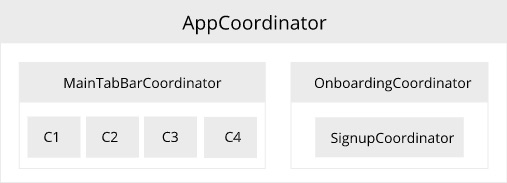
\includegraphics[width=10cm]{qix_coord}
    \captionof{figure}{
       Il Coordinator pattern in QIX
    }
    \label{fig:8}
\end{minipage} \\ \\

Tale struttura è stata creata per permettere modifiche future semplici e scalabili.
Esiste solo un vincolo: deve esistere un rootCoordinator, ossia colui che gestirà il primissimo viewController dell'applicazione, in questo caso è MainTabbarCoordinator ed è il
coordinator che gestirà le animazioni.